\chapter{Erhebung der Anforderungen an das neue Korrelationsformat}\label{ch:anforderungen}


\section{Methode zu Erhebung der Anforderungen}

Zur Herleitung der Anforderungen an das neue Korrelationssystem wird zunächst die proprietäre Produktmodellierung der \metaeffektsp beschrieben, die in den meisten Fällen als Ausgangspunkt der Produktidentifikation dienen wird.
Aus diesem werden die unterschiedlichen relevanten Software-Ökosysteme vorgestellt und wie sich diese in den Software-Inventaren darstellt.
Anschließend wird der intern entwickelten Schwachstellenscanners vorgestellt, und das darin bisher verwendete Korrelationsformat zur Zuordnung von Komponenten mit ihren anderen Repräsentationen.
Das bestehende Format wird anschließend auf seine Schwächen und Herausforderungen untersucht, woraus die Anforderungen an das neue Korrelationsformat abgeleitet werden.


\section{Interne Produktmodellierung der \metaeffektlg}\label{sec:metaeffekt-inventory-format}

Wie alle Datentypen im Inventar basieren auch Artefakte auf Key-Value-Pairs, einer frei definierbaren Zuordnung von Textschlüsseln zu Textwerten.
Dieses Format wurde gewählt, um möglichst einfach Änderungen und neue Felder einführen zu können, ohne Schemata definieren und ändern zu müssen.
Komplexere Werte als flache Texte werden z.B.\ automatisch als JSON-Objekte serialisiert und beim Einlesen wieder als Objekte deserialisiert.

Für Artefakte ist die zugrunde liegende Struktur mit einigen Basis-Feldern für alle Software-Ökosysteme die gleiche, jedoch unterscheidet sich je nach Ökosystem die tatsächliche Verwendung der Felder.
Jedes Ökosystem hat somit eine übliche Menge an Feldern, mit denen eine Komponente beschrieben wird, die typischerweise ausgefüllt werden.

Beispielhafte Artefakte aus dem Java/Maven-Ökosystem sind in \autoref{tab:inventory-artifact-entries} dargestellt.

\begin{table}[ht]
    \caption{Beispielhafte Artefakteinträge in einem Software-Inventar}
    \label{tab:inventory-artifact-entries}
    \centering
    \begin{tabular}{llll}
        \toprule
        \textbf{Id}                  & \textbf{Component}         & \textbf{Group Id}        & \textbf{Version} \\
        \midrule
        commons-codec-1.15.jar       & Apache Commons Codec       & commons-codec            & 1.15             \\
        commons-collections4-4.1.jar & Apache Commons Collections & org.apache.commons       & 4.1              \\
        slf4j-api-1.7.36.jar         & SLF4J                      & org.slf4j                & 1.7.36           \\
        log4j-api-2.14.0.jar         & Apache Log4j               & org.apache.logging.log4j & 2.14.0           \\
        \bottomrule
    \end{tabular}
\end{table}

Da das Datenmodell tabellarisch angeordnet ist und damit in Tabelleneditoren mit mehreren Tabellenblättern abbildbar ist, wird es häufig in menschenlesbarer Form als \texttt{.xlsx} oder ähnlichen Formaten exportiert.

\subsection{Analyse bestehender Softwareinventare}

Da die Darstellungsweisen von Artefakten unterschiedlicher Software-Ökosysteme in den \metaeffekt-Software-Inventaren nicht vollständig normiert sind, wurde ein Datensatz mit den Artefakten aus 1820 realen Software-Inventaren von unterschiedlichen Quellen in einer Datenbank aggregiert und auf Muster untersucht.
Es stellt sich heraus, dass in den meisten Fällen die Art eines Artefakts durch eine Kombination von drei Attributen ableiten lässt: \texttt{Type}, \texttt{Component Source Type} und \texttt{Ecosystem}.
Nicht immer sind alle gesetzt, und manchmal kommt es auf die Kombination mehrerer an.

Das Attribut \texttt{Ecosystem} in Artefakten entspricht dem \texttt{type}-Attribut in \acrshortpl{purl} und kann von den erzeugenden Prozessen nur dann aufgefüllt werden, wenn auch eine \acrshort{purl} angegeben ist.
Fehlt dieses, kann meist \texttt{Component Source Type} für eine allgemeine Klassifikation und \texttt{Type} für die spezifischere Einordnung in ein zweistufiges hierarchisches Modell verwendet werden.
Leider wurden in dem Datensatz oft Artefakte komplett ohne Typ-Information gefunden, in diesen Fällen müssen weitere Algorithmen zur Erkennung etwa basierend auf Dateiendungen oder anderen Attributen entwickelt werden.

Ein Auszug aus den Werten des \texttt{Ecosystem}-Attributs:
\texttt{npm}, \texttt{gem}, \texttt{github}, \texttt{cpan}, \texttt{wut}, \texttt{docker}, \texttt{internal}, \texttt{conan}, \texttt{deb}, \texttt{nuget}, \texttt{generic}, \texttt{maven}, \texttt{rpm}, \texttt{pypi}, \texttt{golang}, \texttt{apk}.

Die beobachteten Werte aus den Attributen \texttt{Component Source Type} und \texttt{Type} reichen von Ökosystemen und Dateitypen bis hin zu Begriffen aus der Betriebssystem- und Gerätetreiberdomäne.
Da sich einige Typen in unterschiedlichen Schreibweisen oder Bedeutungen wiederholen, kann von einer stark heterogenen Entstehung der Artefakte ausgegangen werden.
Die folgenden Kombinationen aus \texttt{Component Source Type} und \texttt{Type} konnten im Datensatz gefunden werden:

\begin{itemize}
    \itemsep0em
    \item \texttt{generic-version → package}
    \item \texttt{java-runtime → package}
    \item \texttt{pwa-module → web-module}
    \item \texttt{bower-module → web-module}
    \item \texttt{npm-module → nodejs-module, web-module}
    \item \texttt{jar-module → module}

    \item \texttt{<empty> → (hardware/drivers) storage controller, imaging hardware, operating-system, audio hardware, power driver, mouse, Universal Serial Bus controller driver, data storage, multimedia output device, device connector, firmware driver, storage driver, printer driver, power supply, extension module, disk drives driver, printer, input device, audio driver, computer driver, display driver, processing core, driver, sensor, multimedia driver, appliance, security token, sound hardware, network driver, mouse driver, usb controller driver, security device driver, Bluetooth driver, keyboard, controller, operating system, display, imaging driver, port driver, security hardware, input device driver, system device driver, keyboard driver, print queue driver, processor driver, software device driver, networking hardware, board}
    \item \texttt{<empty> → (other) package, python-module, nodejs-module, bios, file}
    \item \texttt{<empty> → <empty>}
\end{itemize}

Bei einer Sichtung des Quellcodes einiger Entstehungsquellen von Artefakten konnte die große Auflistung der Hardware- und Betriebssystemtypen in dem Windows-Inventar-Extraktor System gefunden werden, die restlichen sind über diverse Extraktoren verteilt oder werden extern aufgefüllt und damit nicht einheitlich nachvollziehbar.

% erkennungsrichtlinien für einzelne ökosysteme


\section{Analyse des Schwachstellenscanners der \metaeffektlg}

% “The results show that the method describe” (Sanguino and Uetz, 2017, p. 22) Sanguino_Uetz_2017
%   auf diese art und weise die shortcomings unseres scanners beschreiben
% vor allem problematisch wenn es keine CPE gibt weil dann oft doch eine gefunden wird
% subsection über effective CPE

\subsection{Effective CPE Calculation}\label{subsec:effective-cpe-calculation}


\section{Aktuelles Korrelationsformat zur Modifikation von Artefaktmetadaten}\label{sec:current-correlation-format}

Das Korrelationsformat wurde 2021 entwickelt, um manuelle Nachkorrekturen an den durch die \enquote{CPE Derivation} automatisch abgeleiteten \acrshort{cpe}-Identifikatoren zu ermöglichen.
Während der Hauptanwendungsfall daraus besteht, fehlerhafte oder unpassende \acrshort{cpe}-Zuordnungen zu korrigieren, ermöglicht es die Modifikation beliebiger Artefaktattribute, und wurde so über die Zeit für viele weitere Anwendungsfälle eingesetzt.

Das Format basiert auf \acrfull{yaml} und folgt einem zweistufigen Modell:
Über einen Selektor werden Regeln für die Auswahl von Artefakten definiert, und dann eine Reihe an Modifikationen, die an diesem Artefakt vorgenommen werden sollen.
Jeder Korrelationseintrag kann aus den folgenden Attributen bestehen, wobei mindestens ein \texttt{affects} und eine Modifikationsoperation definiert sein muss.
Ein kleines Beispiel bei dem eine \acrshort{cpe} zu einem Artefakt hinzugefügt wird kann in \autoref{lst:correlation-initial-example} gefunden werden, ausführlichere Beispiele mit Beschreibungen werden nach der Formatbeschreibung aufgeführt.

\begin{lstlisting}[style=yaml,caption={Korrelationseintrag für die Java-Komponente Liquibase},label={lst:correlation-initial-example}]
- affects:
    - Id: liquibase-*.jar
    - Id: org.liquibase.liquibase-*.jar
  append:
    Additional CPE URIs: cpe:/a:liquibase:liquibase
\end{lstlisting}

\paragraph{Artefakt-Selektion}
Die \texttt{affects}-Sektion eines Eintrages muss immer vorhanden sein und legt fest, auf welche Artefakte sich der Eintrag beziehen soll.
Dabei wird in einer Listenstruktur eine Menge an Attribut-Wert-Paaren angegeben, die auf der Ebene der Liste logisch als ODER-Verknüpfung interpretiert werden und die Attribute innerhalb der Liste mit einer UND-Verknüpfung verbunden sind.
Das bedeutet, dass bereits ein zutreffendes Listenelement ausreicht, um einen Treffer zu erzielen, aber innerhalb jedes Elements müssen alle angegebenen Attribut-Werte-Paare auf das zu prüfende Artefakt zutreffen.
Die betroffenen Attribute können beliebige Felder aus einem Artefakt sein (etwa \texttt{Id}, \texttt{Component}, \texttt{Group Id}, \texttt{Type}, \ldots).
Es ist dadurch möglich domänenübergreifende Selektionskriterien zu formulieren.

Optional kann ein \texttt{ignores}-Block definiert werden, der vom Aufbau her der \texttt{affects}-Sektion entspricht, aber die Logik umkehrt.
Sobald einer der Listeneinträge mit einem Artefakt erfolgreich verglichen wurde, wird das Artefakt von dem Eintrag ausgeschlossen.
Damit können Ausnahmen und Abgrenzungen zu ähnlichen Artefakten erstellt werden, etwa bei Artefakten mit ähnlichen Namen aber unterschiedlichen Ökosystemen.

Die zu vergleichenden Werte der Attribut-Wert-Paare unterstützen mehrere Matching-Modi.
Im einfachsten Fall wird ein Text auf Gleichheit mit dem Attributinhalt verglichen, hierzu wird der Text einfach aufgeführt.
In diesem einfachen Vergleichsmodus können Platzhalterzeichen verwendet werden, so steht ein Sternchen (\texttt{*}) für beliebig viele Zeichen und ein Fragezeichen (\texttt{?}) für ein einzelnes beliebiges Zeichen.
Über zwei Stufen können sich die Werte regulären Ausdrücken annähern:
Ähnlich zu der Notation wie sie in JavaScript verwendet wird \autocite{MdnRegularExpressions2025} können durch das Anhängen von einem Schrägstrich und einer Menge an Flags wie in \enquote{\texttt{/i}} beispielsweise auch case-insensitive Vergleiche durchführen, ohne vollständig auf reguläre Ausdrücke zu wechseln.
Die vollständige Nutzung von regulären Ausdrücken wird ermöglicht, wenn das Muster von vorne und hinten durch \enquote{\texttt{/}} eingerahmt wird.
Durch diese inkrementelle Syntax kann einfach zwischen unterschiedlichen Matching-Modi gewählt werden.

\paragraph{Artefakt-Modifikation}
Sobald ein Artefakt durch einen Eintrag als betroffen erkannt wird, werden die im zweiten Teil des \acrshort{yaml}-Blocks definierten Modifikationen angewandt.
Auch hier gibt es unterschiedliche Weisen, die Attribute der Artefakte zu modifizieren, wobei sich das allgemeine Schema bei den meisten gleicht:
Jede Art an Modifikation führt eine Menge an Attributen, die jeweils einen Text-Wert zugeordnet haben.
Die am häufigsten verwendete Operation ist \texttt{append}, die auf \acrfull{csv}-Attributen angewendet wird, und den angegeben Wert entweder mit einem Komma getrennt an den vorhandenen angehängt wird, oder direkt gesetzt wenn noch keiner vorhanden ist.
Typischerweise betrifft dies \acrshortpl{cpe}, die nachträglich als gültig oder unpassend erkannt wurden und zu einer entsprechenden Liste hinzugefügt werden sollen.
Ähnlich operiert \texttt{remove}, womit auch hier der auf dem Artefakt vorhandene Wert und der im Korrelationseintrag angegebene Wert als \acrshort{csv}-Werte interpretiert und an Kommas getrennt werden und die Schnittmenge der beiden Listen vom Artefakt-Attribut entfernt werden.
\enquote{overwrite} ersetzt den kompletten Inhalt eines Attributs mit einem neuen Werte und \enquote{clear} entfernt ein Attribut von einem Artefakt.

\bigskip

Mit diesen Methoden, auf Artefakte zuzugreifen, können potenziell alle Transformationen an Artefakten durchgeführt werden, die von Interesse sind.
Im Kontext der \acrshort{cpe}-Zuordnung sind besonders die drei Felder relevant, die auch schon in \autoref{subsec:effective-cpe-calculation} aufgeführt wurden:
\texttt{Additional CPE URIs}, \texttt{Inapplicable CPE URIs} und \texttt{CPE URIs}.

Ein Konsens, der sich über die Zeit aus Gründen der Nachvollziehbarkeit geformt hat, ist das Hinzufügen eines Kommentarblocks vor dem Korrelationseintrag mit Informationen über das Artefakt, für den der Eintrag angelegt wurde und eine Begründung, warum er nötig ist.
Dieser Kommentar kann beliebige Begründungen enthalten, etwa Verweise auf Dokumentationen, URLs zu Projektseiten oder kurze Erklärungen, warum etwa eine bestimmte \acrshort{cpe} als passend oder unpassend eingestuft wurde.
Bei späteren Revisionen und Diskussionen im Team erleichtert das die Nachvollziehbarkeit vergangener Entscheidungen.

\paragraph{Inkrementelle Korrelationseinträge}
werden ermöglicht, da für ein Artefakt alle Korrelationseinträge im Datensatz ausgewertet werden und nicht einfach bei einem ersten zutreffenden gestoppt wird.
Dadurch können aufeinanderfolgende Korrelationseinträge definiert werden, die nacheinander auf ein Artefakt angewendet werden, um einen gewünschten Effekt zu erzielen.

Ein beispielhafter Anwendungsfall betrifft Artefakte mit dem Namensbestandteil \enquote{git} (vgl. \autoref{lst:correlation-incremental-git-example}).
Oft wird auf Artefakten die \acrshort{cpe} \texttt{cpe:/a:github:github} durch die CPE URI Derivation automatisch hinzugefügt, die den Text-Schnipsel \texttt{git} in ihrem Namen enthalten.
Oft wird durch die automatische \acrshort{cpe} URI Derivation die \acrshort{cpe} \texttt{cpe:/a:github:github} zugewiesen, die den GitHub Enterprise Server\footnote{\url{https://docs.github.com/en/enterprise-server/admin/all-releases}} referenziert.
Dieser kann allerdings auf diese Weise nicht in den Software-Inventaren der \metaeffektsp vorkommen kann, deaktiviert ein generischer Eintrag diese \acrshort{cpe} für alle Artefakte, die \enquote{git} in egal welchem Attribut enthalten.
Ein spezifischer Folgeeintrag darunter führt die tatsächliche \texttt{git}-Kommandozeilenapplikation auf, bei der dann die falsche \texttt{cpe:/a:github:github} nicht mehr behandelt werden muss, sondern nur noch die konkreten git-spezifischen \acrshortpl{cpe} aufgeführt werden können.

So können allgemeine Muster an einer Stelle behandelt werden und artefaktspezifische Regeln ohne diese isoliert aufgeführt werden können.
Diese Trennung verhindert Redundanzen und vereinfacht spätere Anpassungen.
In \autoref{fig:correlation-utilities-demo} können oben rechts weitere Beispiele dieser allgemeinen Einträge gefunden werden.

\begin{lstlisting}[style=yaml,caption={Inkrementelle Korrelationseinträge für das Kommandozeilentool git},label={lst:correlation-incremental-git-example}]
- affects:
    - any: "*git*/i"
  append:
    Inapplicable CPE URIs: cpe:/a:github:github

- affects:
    - Component: git
      Type: package
  append:
    Inapplicable CPE URIs: cpe:/a:codesys:git, cpe:/a:cygwin:git, cpe:/a:git:git-shell, cpe:/a:gitforwindows:git, cpe:/a:jenkins:git
    Additional CPE URIs: cpe:/a:git:git, cpe:/a:git-scm:git, cpe:/a:git_project:git
\end{lstlisting}

\subsection{Beispiele zu Korrelationsdaten}

\paragraph{Beispiel 1: snappy-1.1.8}
In \autoref{lst:correlation-snappy} ist ein Beispiel aufgeführt, bei dem ein Artefakt \texttt{snappy-1.1.8} als ein Linux Package (Typ \texttt{package}) in einem Softwareinventar identifiziert wurde.
Der CPE URI Derivation-Algorithmus hat in das Attribut \texttt{Derived CPE URIs} seine Identifikation aufgenommen, nämlich \texttt{cpe:/a:knplabs:snappy}.
Vom Namen her sieht diese Identifikation vielleicht überzeugend aus, allerdings stellt sich dies als eine Fehlidentifikation heraus, denn die \acrshort{cpe} verlinkt in ihren Metadaten auf \url{https://github.com/KnpLabs/snappy}, was eine PHP Bibliothek ist und kein Linux Paket.
Erst bei einer manuellen Suche kommt eine zweite \acrshort{cpe} hervor, \texttt{cpe:/a:google:snappy}, die tatsächlich ein Linux Paket darstellt welches nicht nur vom Namen her passt, sondern auch von der Versionsreichweite der veröffentlichten Versionen.
Allerdings wurde auch eine Java-Bibliothek mit demselben Namen identifiziert, also mussten die entsprechenden jar-Dateien über \texttt{ignores} ausgeschlossen werden.
Alternativ hätte auch das \texttt{affects} mit \texttt{Type: package} erweitert werden können, um die Artefakte so zu limitieren.
So ergibt sich der gesamte Eintrag, in dem allgemein alle mit \texttt{snappy-} startenden Artefakte ausgewählt werden, die mit \texttt{.jar} hinten exkludiert und auf den Restlichen die jeweiligen \acrshortpl{cpe} als anwendbar oder nicht in die Artefakt-Attribute mit aufgenommen werden.
In der Praxis würde nun noch ein weiterer Eintrag für die PHP-Bibliothek angelegt werden, der auf den korrekten \texttt{Type} prüft.

\begin{lstlisting}[style=yaml,caption={Korrelationseintrag für Snappy-Komponenten},label={lst:correlation-snappy}]
# Id: snappy-1.1.8
# Component: snappy
# Version: 1.1.8
# Type: package
# Derived CPE URIs: cpe:/a:knplabs:snappy
# reason:
#   cpe:/a:knplabs:snappy --> https://github.com/KnpLabs/snappy --> "PHP library allowing thumbnail, snapshot or PDF generation from a url or a html page." --> PHP library
#   cpe:/a:google:snappy --> https://github.com/google/snappy --> https://pkgs.alpinelinux.org/package/edge/main/x86/snappy --> linux package --> matches this package version range
#   ignore https://mvnrepository.com/artifact/org.xerial.snappy/snappy-java
- affects:
    - Id: snappy-*
  ignores:
    - Id: snappy-*.jar
  append:
    Inapplicable CPE URIs: cpe:/a:knplabs:snappy
    Additional CPE URIs: cpe:/a:google:snappy
\end{lstlisting}

\paragraph{Beispiel 2: Microsoft Windows 10 (Version 21H2)}
Auch nicht-\acrshort{cpe}-Attribute können auf Artefakten ergänzt werden.
In dem Beispiel in \autoref{lst:correlation-win-10-21H2} wird eine Microsoft-Produkt-Id zu dem Betriebssystem Windows 10 in der Version 21H2 zugeordnet.
Der \href{https://github.com/org-metaeffekt/metaeffekt-documentation/blob/bd184b2889d5421b5a71dcd26c1ac0ffc63d07e7/metaeffekt-vulnerability-management/data-mirror/msrc/understanding-data.md}{Dokumentationeintrag zu den Microsoft-Datenquellen} und in \autoref{subsec:msrc-product-ids} wird das Microsoft-Produktidentifikator-Ökosystem näher erklärt, aber prinzipiell haben alle versionierten Produkte in der Microsoft-Datenbank eine eindeutige numerische Id, unter der Schwachstellen registriert werden.
Daher muss nur auf die exakten Attribute geprüft werden und dann kann die korrekte Produkt-Id zu dem Artefakt hinzugefügt werden.
Zusätzlich wird für das EOL-Ökosystem die entsprechende Produkt-Id \texttt{windows} hinzugefügt und eine für die Abfrage spezifische Version die in diesem Ökosystem verwendet werden muss.

\begin{lstlisting}[style=yaml,caption={Korrelationseintrag für Snappy-Komponenten},label={lst:correlation-win-10-21H2}]
# reason: https://learn.microsoft.com/de-de/windows/release-health/release-information
#   11931 --> Version 21H2 (OS build 19044) / Windows 10 Version 21H2 for x64-based Systems
- affects:
    - Id: Microsoft Windows 10*
      Version: 10.0.19044*
      Type: operating system
      Architecture: "*64*"
    - Id: Windows 10*
      Version: 10.0.19044*
      Type: operating system
      Architecture: "*64*"
  append:
    MS Product ID: "11931"
    EOL Id: windows
    EOL Overwrite Cycle Query Version: 10 21H2 (E)
\end{lstlisting}

\subsection{Correlation Utilities als Tool zur Korrelationsarbeit}

Die \enquote{Correlation Utilities} sind ein spezialisiertes Experten-Werkzeug zur Analyse von Software-Inventaren im Rahmen der Erstellung und Pflege von Korrelationsdaten.
Ein Software-Inventar mit dem Ziel der korrekten Schwachstellenzuordnung manuell durchzuarbeiten ist ein komplexer und zeitintensiver Prozess.
Die Correlation Utilities stellen eine dedizierte Benutzeroberfläche dar, mit der die spezifischen Aufgabenbereiche dieser Arbeit unterstützt werden.

Technisch besteht das Werkzeug aus einer Spring-Boot-basierten Backend-Anwendung und einem Frontend, das über kachelartige Widgets dynamisch vom Nutzer angeordnet werden kann.
Eine typische Sitzung beginnt mit der Auswahl eines Inventars und dem automatisierten Anreichern von Schwachstellinformationen und begibt sich dann auf den Prozess, jedes Artefakt in dem Inventar auf seine \acrshort{cpe}-Zuordnungen einzeln zu prüfen und Korrekturen durch das Anlegen von neuen Korrelationseinträgen vorzunehmen.

In \autoref{fig:correlation-utilities-demo} kann eine beispielhaft angeordnete Nutzeroberfläche gesehen werden.
Die Benutzeroberfläche in dieser Anordnung besteht links oben aus der Tabelle der Artefakte, mit farbigen Status-Indikatoren pro Zeile um schnell nach relevanten Metriken filtern zu können.
Links unten ist ein Widget zu sehen, das eine Detailsicht mit allen Attributen des aktuell ausgewählten Artefakts anzeigt.
Hier werden zudem über Web-Requests und lokale Datenbankabfragen diverse weitere Informationen, Links und Internetsuchen aggregiert und für den Nutzer vorbereitet.

\begin{figure}
    \centering
    \makebox[\linewidth]{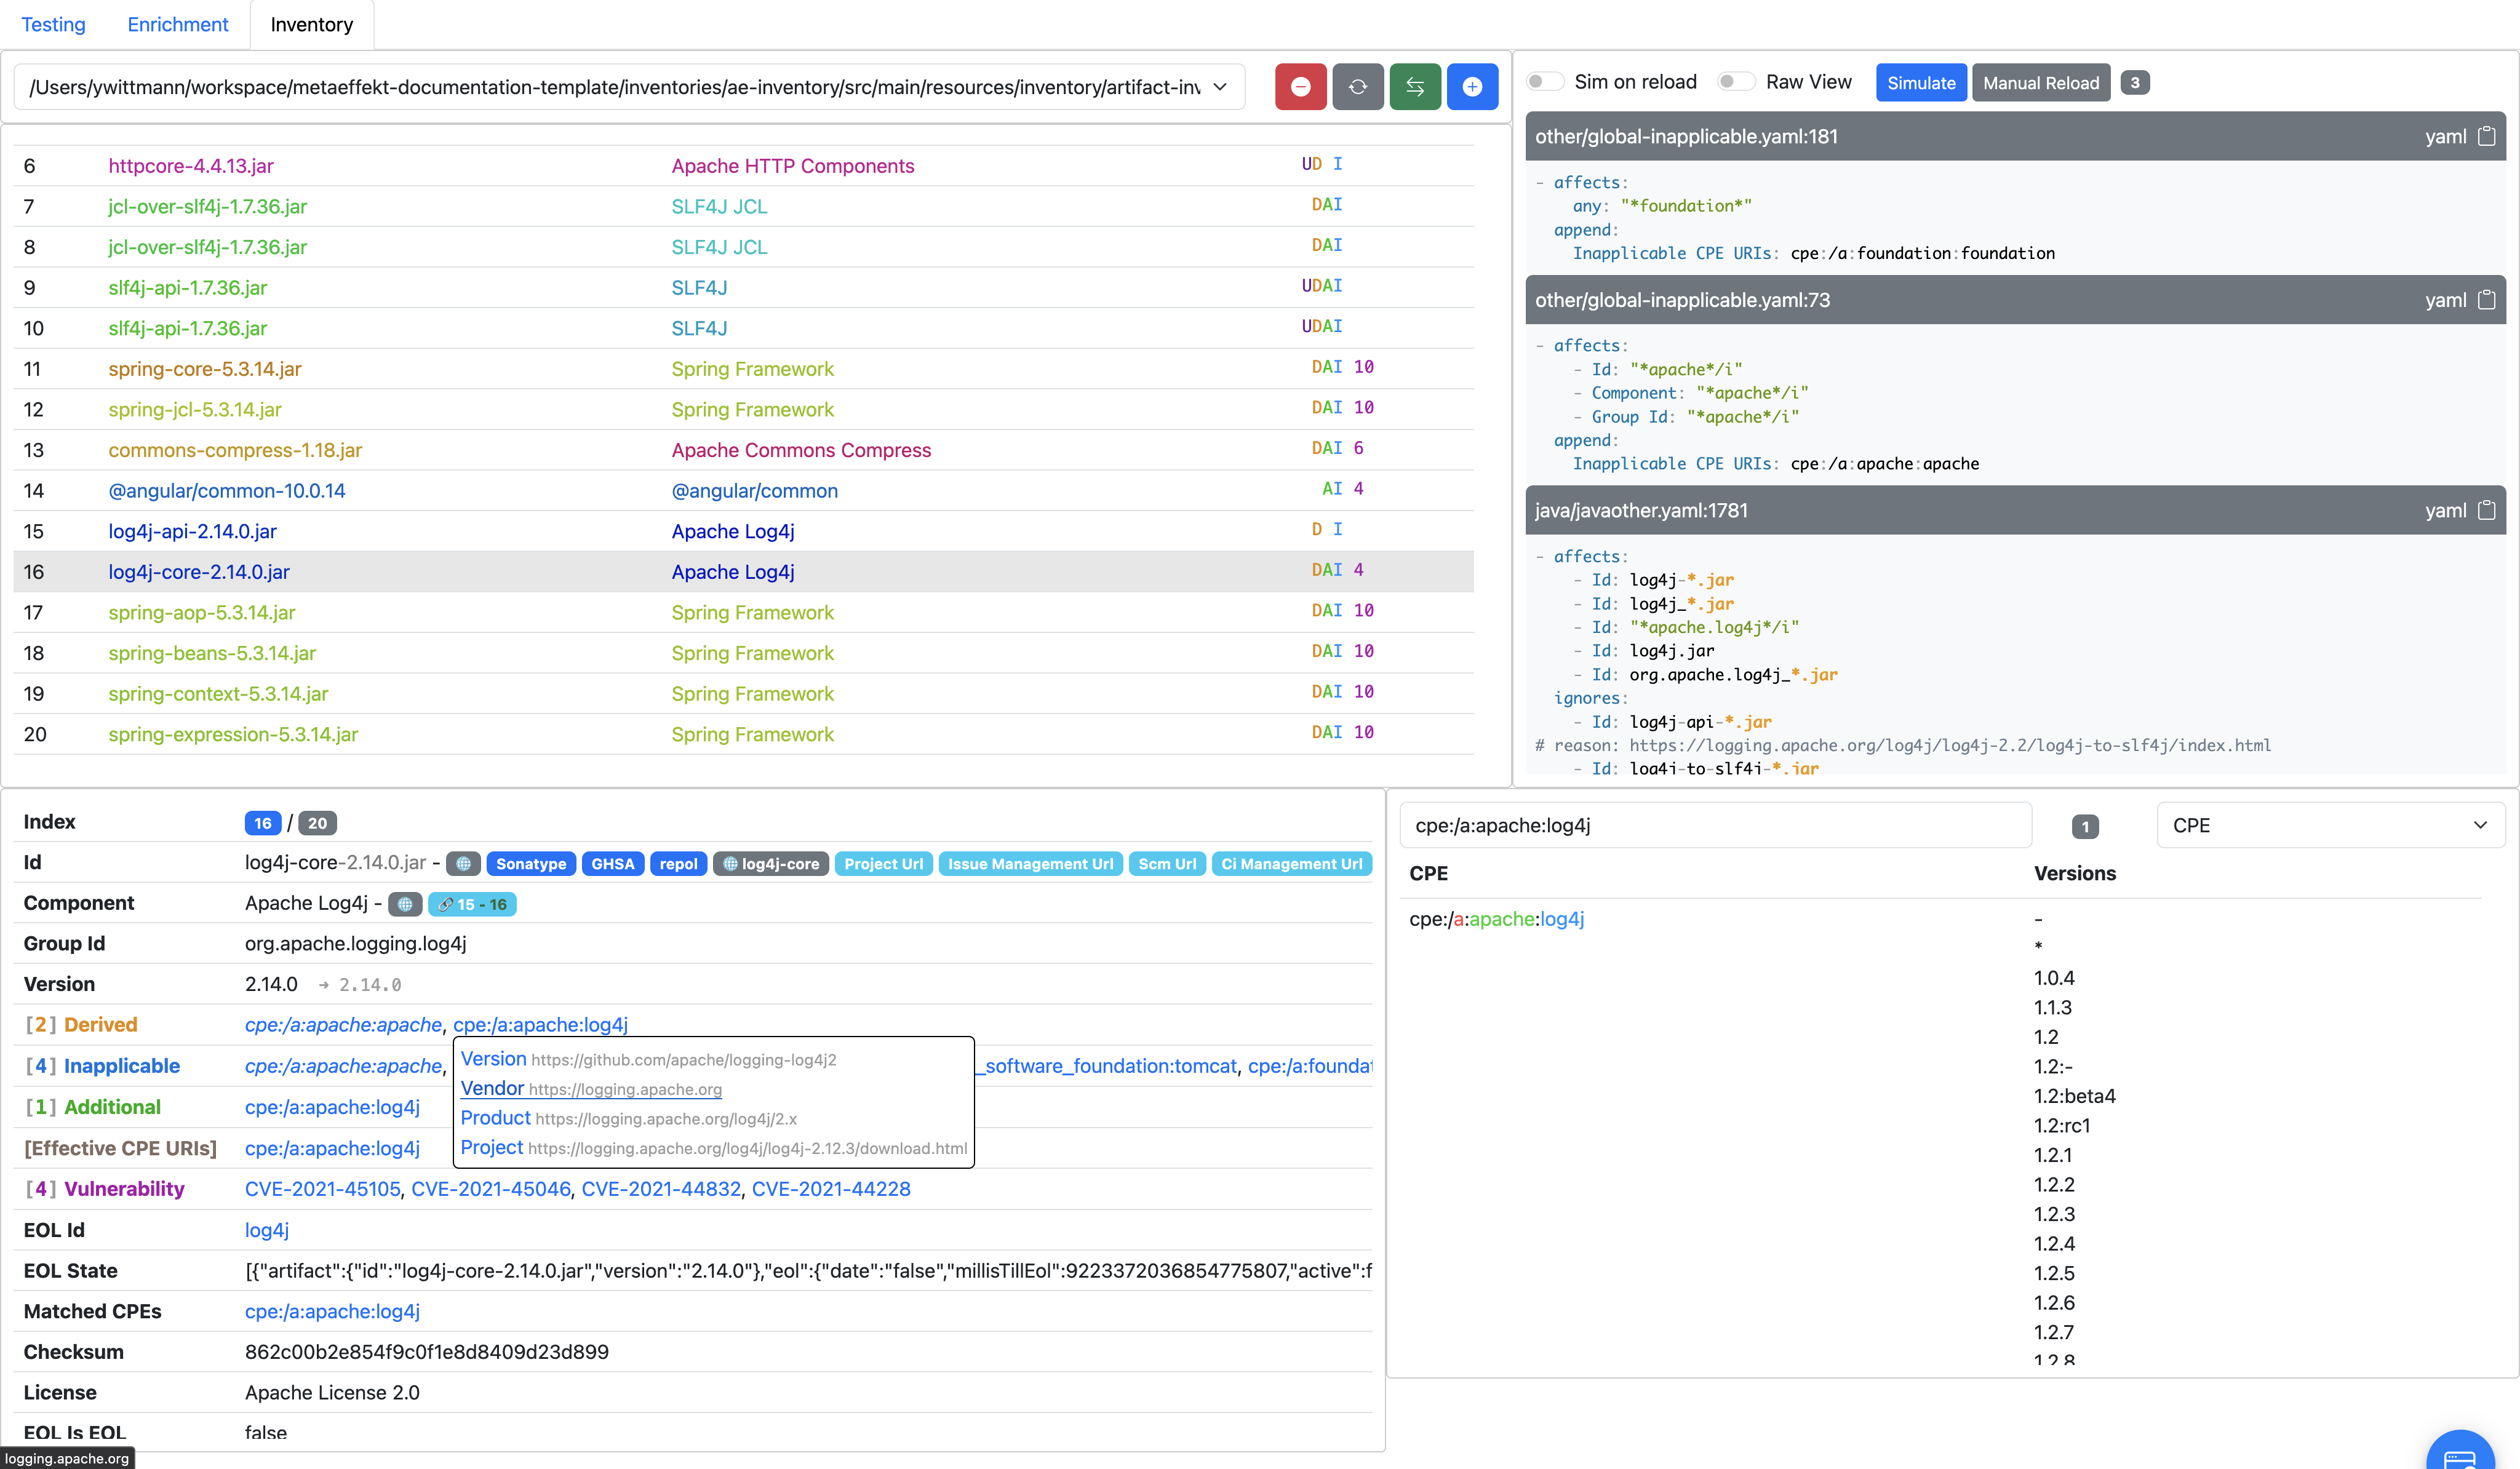
\includegraphics[keepaspectratio,width=1.3\linewidth]{../../images/correlation-utilities-demo}}
    \caption{Das Artefakt \texttt{log4j-core-2.14.0.jar} in den Correlation Utilities}
    \label{fig:correlation-utilities-demo}
\end{figure}

Ein weiteres Widget auf der rechten Seite zeigt, welche Korrelationseinträge auf das aktuelle Artefakt angewendet wurden und erlaubt über eine Integration mit IntelliJ IDEA den direkten Zugriff auf die Korrelationseinträge im Editor und schlägt auf der Basis von einigen bekannten Mustern neue Einträge vor, die mit einem Klick übernommen werden können.
Die Korrelationseinträge werden automatisch bei Änderungen in den Dateien neu geladen und ausgewertet.
Unten rechts kann eine integrierte Abfrageschnittstelle zu den lokalen Datenbanken gefunden werden, über die Abfragen etwa zu \acrshortpl{cpe}, \acrshortpl{cve} oder Produktversionen getätigt werden können.

% TODO: actually perform test, ask Julian
% \smallskip
% Nach einem internen Test hat sich herausgestellt, dass Mitarbeiter mit den Utilities mehr als 2.5-mal so schnell dieselbe Arbeit in höherer Ergebnisqualität durchführen konnten, wie wenn sie dieses Tool nicht verwendet hätten.

\paragraph{Fallunterscheidungen je Artefakt}
Für den allgemeinen Arbeitsablauf mit diesem Tool gibt es pro Artefakt mehrere Fälle, die auftreten können:

\begin{itemize}
    \item Wenn das Artefakt \enquote{Derived CPE URIs} hat, die nicht von einem der weiteren \acrshort{cpe}-Attribute (Additional, Ignores, \ldots) abgedeckt sind, dann bedeutet dies, dass die \acrshortpl{cpe} noch nicht manuell behandelt und geprüft wurden.
    Diese Art von \acrshort{cpe} auf einem Artefakt nennt sich im Tool \enquote{Untouched CPEs}.
    Nachdem sie auf ihre Richtigkeit geprüft wurden, muss die Entscheidung über einen vorhandenen oder neuen Korrelationseintrag in einem der manuellen \acrshort{cpe}-Attribute festgehalten werden.
    Doch nicht nur die automatisch hinzugefügten \acrshort{cpe} müssen untersucht werden, es muss auch nach zusätzlichen \acrshortpl{cpe} im Internet oder den lokalen Datenbanken gesucht werden, um sicherzustellen, dass alle korrekten \acrshort{cpe} gefunden werden.

    \item Wenn das Artefakt nur manuelle \acrshort{cpe}-Attribute gesetzt hat, dann handelt es sich bei diesem Artefakt um ein bereits bekanntes, welches in der Vergangenheit einmal bearbeitet wurde.
    In den meisten Fällen ist hier keine neue Arbeit nötig.
    Manchmal jedoch gibt es Fälle, in denen ein Artefakt seit der letzten Analyse eine neue \acrshort{cpe} zugewiesen bekommen hat, etwas bei dem vorherigen Durchgang übersehen wurde, oder es sich um eine Fehlidentifikation in den Korrelationsdaten handelt und diese fehlerhaft hinzugefügt wurde.
    Je nach Attribut-Kombination sind unterschiedliche Fälle wahrscheinlicher, für welche eine Person mit der Zeit ein Gefühl bekommt.

    \item Wenn das Artefakt überhaupt keine \acrshort{cpe}-Information hat, dann muss manuell nachgeprüft werden, ob es zusätzliche gibt, die diesem Produkt entsprechen.
    Wenn eine oder mehrere passende gefunden werden, wird mit diesen ein neuer Korrelationseintrag angelegt.
\end{itemize}

Vor allem bei einem ersten Durchlauf eines Software-Inventars treten die ersten beiden Fälle häufig auf, aber auch bei erneuten Analysen bekannter Inventare müssen die Artefakte auf ihre Richtigkeit geprüft werden.


\section{Schwächen und Herausforderungen des aktuellen Korrelationsformats}

\subsection{Unspezifische Identifikation von Artefakten}

% Currently, there are many entries (almost all) that rely on the * wildcard in the Id field to match components version-agnostically. This is not a maintainable approach, since shorter or more common identifiers tend to either be overloaded with multiple components sharing a name, or beginning with the other’s full name. For example:
% - affects:
%     - Id: auth-*.jar
%
% would not only affect an artifact auth-1.2.3.jar, but also auth-registration-helpers-1.2.3.jar. To currently mitigate this, an ignores entry has to be added to the original entry for every single one of these cases.
% - affects:
%     - Id: auth-*.jar
%   ignores:
%     - Id: auth-registration-helpers-*.jar
%
% Fields like the Component cannot be used reliably, since they are often hand-filled or not standardized. Fields like the PURL are more common these days, but still not available on every generated inventory. The artifact Type is still not a normalized field, although it hopefully soon will be (
% AE-556: [Artifact Analysis] Define [Artifact Type] / [Component Source Type], create Data Types and apply consistently across code baseTo Do).
% It would be nice if there was a smarter preprocessing step, that would attempt to recover this kind of information in a normalized way, based on several different criteria. The ones listed below are merely examples to illustrate what could be done, this is to be defined:
%     Actual component name
%         Check if there is a PURL and whether it matches with either Component or the Id
%         Check whether the Id contains the Component
%         Fallback to Id
%     Actual component type / ecosystem
%         Consists of a component category (web-module) and a subcategory (nodejs-module)
%         This will be available more generally in the future, but for now this information would have to be guessed from the available fields Type, PURL, etc.
%         This information would be very useful to limit the matching of an entry to a single ecosystem, without affecting others.
%     Version
%         The version field is already fairly normalized, but maybe add a nicer way to compare versions with the component version instead of the huge entry that is currently required for this
% These computed values can be used in the component identification as listed below to reduce the ambiguity in matching and reduce the complexity of the data.
%
% Basically: Enable better, ecosystem-specific matching of artifacts.
% Simply to get the idea across, something like this:
% - affects:
%   - matcher type: maven
%     group id: com.x
%     artifact id: some-artifact

\subsection{Duplizierte Artefakt-Selektoren}

% doppelt weil aufeinander aufbauende einträge
% wenn ein feld unterschiedlich gleich neuer eintrag
%   vererbung als lösung

\subsection{Große und unübersichtliche YAML-Dateien}

% Find a way to better split the entries into multiple files. The 6000-lines files are not only tedious to work with, but also require unnecessarily large amounts of computational power to render, with a notable slowdown of the IDE in use.
% Maybe, as suggested below, YAML files could not even be required for this, maybe another data format would be better suited. We will see.

\subsection{Begründung wird oft nicht ausgefüllt, ist nicht spezifisch genug um sie nachzuvollziehen und nicht maschienenlesbar}

% The current “reason” format is a simple, unstructured text comment. It is not machine-readable or evaluate-able in any way.
% The current format has a loosely defined arrow reasoning chain syntax that looks like this (fake values) cpe:/a:apache:commons_io --> https://github.com/apache/commons-io --> "library for doing IO operations" --> same library as artifact
% Since the content is only a simple text comment in a YAML file, it is impossible for the parser to extract this information and use it somehow to generate more descriptive views on the reason a connection between components and product identifiers has been made.
% This new format should therefore be in a machine-readable format inside the data structure of the connections. This makes it harder for a human correlation assistant to create the data, therefore the user should not have to edit this reason manually, but rather via a UI that they can click “apply” on or similar.

\subsection{Fälle ohne Aktion können nicht dokumentiert werden}

% If an artifact lacks any CPE or other identifiers, a correlation assistant may have already put in significant effort to reach this point. He might have had to make quite the research or other logical conclusions.
% But, in the current system, such cases \textit{cannot} at all be put into the correlation files. A separate (non-normalized or used) file would have to be used to keep this knowledge. But such an additional system does not exist yet, so nothing is done to document the effort and the information is lost.
% The next time a person sees this artifact and either does not remember the effort from last time, or is a completely new person with a fresh perspective, they cannot build on the research that was already made.

\subsection{Schlechtes Testframework, wenig Unterstützung für automatisierte Kontrolle}

% The current correlation system does have a “validation” format that allows for the manual creation of test cases for the created correlation entries, but it’s quite tedious to use.
% It would be much nicer, if the system used to create the correlation data (e.g. correlation utilities) would automatically (or with the press of a button) record the artifact the correlation was created on, the before and after states and create a test case with an expected result based on that.
% Through the more documentation-heavy new format, these tests may also already be self-documenting.

\subsection{Generierte YAML-Dateien}

% The generated directory contains several automatically generated YAML correlation files, based on the data that is present in the index when generating.
% These need to be converted into the new format somehow.

% \subsection{Reihenfolge-Abhängige Anwendung von Einträgen}


\section{Auflistung der Anforderungen}

% “4.3. Data Types in Falcon” ([Cheramangalath et al., 2016, p. 6](zotero://select/library/items/4DG8G9J3)) ([pdf](zotero://open-pdf/library/items/QNYKYEH4?page=6&annotation=C7MKFAUG))
